\begin{figure*}[!htbp]
    \centering
    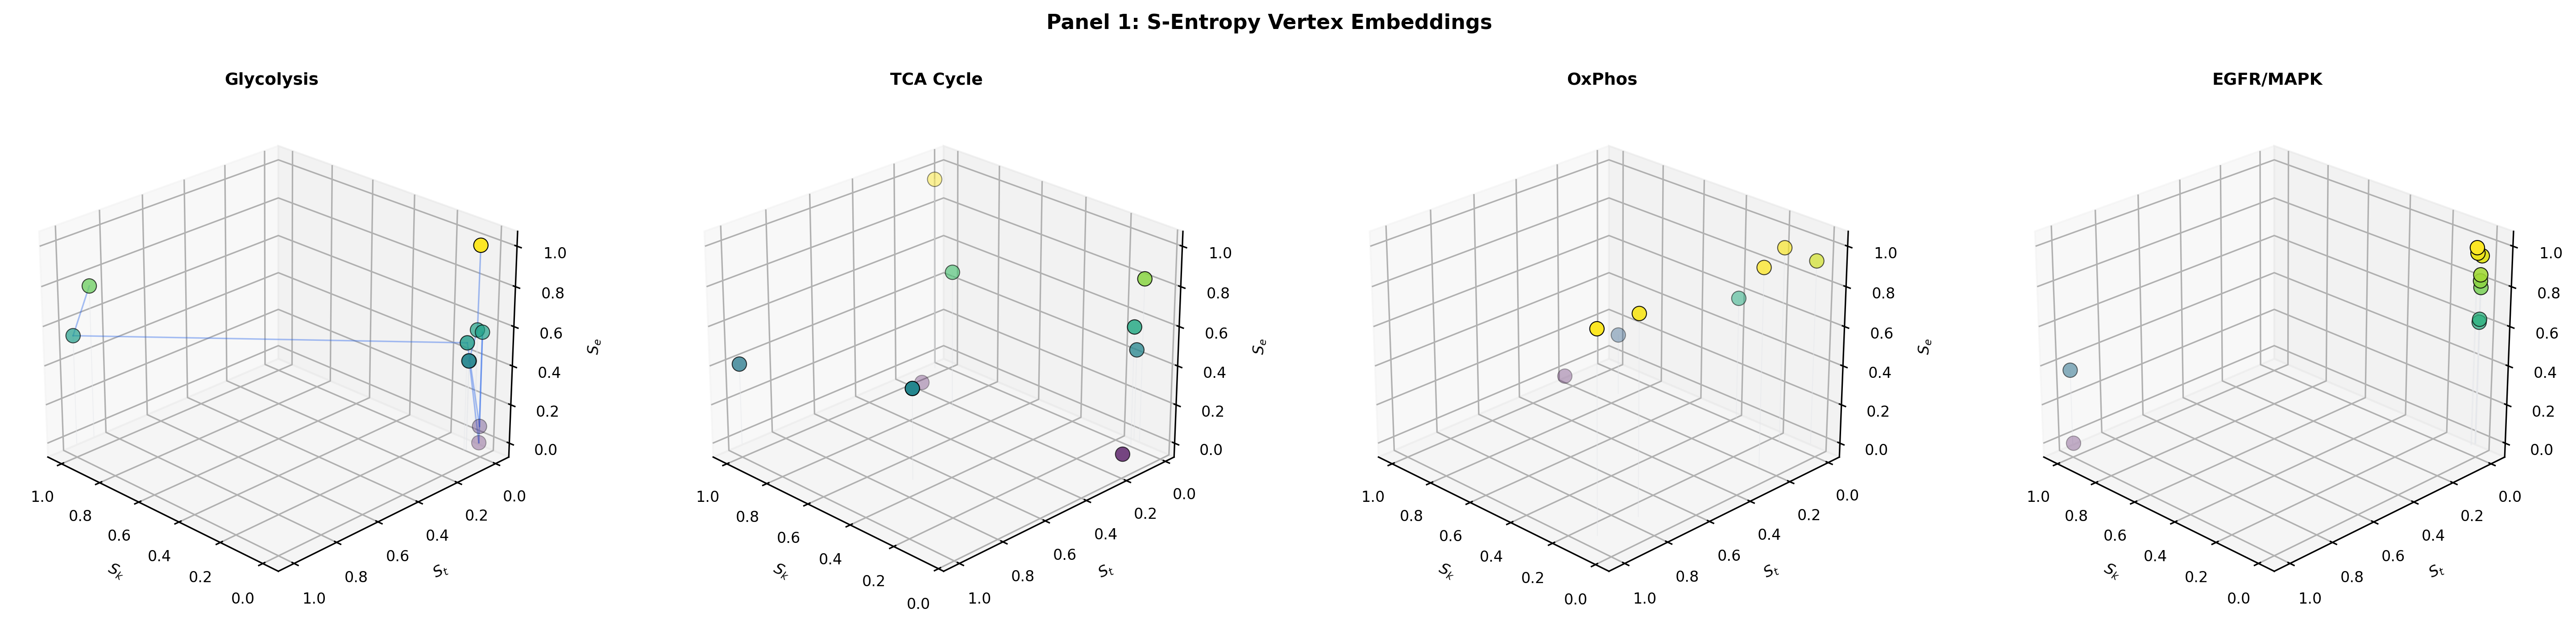
\includegraphics[width=\textwidth]{figures/panel_1_sentropy_embeddings.png}
    \caption{\textbf{S-entropy vertex embeddings $\mathbf{S}: V \to [0,1]^{3}$ for four canonical biochemical networks.}
    Each subplot displays the three-dimensional embedding of every vertex (molecular species) in the S-entropy state space $(\Sk, \St, \Se)$, with colour mapped to the energetic coordinate $\Se$ (viridis scale). Vertical drop lines project each vertex onto the $(\Sk, \St)$ floor to aid depth perception.
    (\textbf{A})~Glycolysis ($P_{10}$, 10 vertices): the preparatory-phase vertices (Glucose, G6P) occupy the high-$\Sk$ region while payoff-phase vertices (3PG, 2PG, Pyruvate) cluster near the origin, reflecting the asymmetric distribution of kinetic flux.
    (\textbf{B})~TCA cycle ($C_9$, 9 vertices): the cyclic topology distributes vertices more uniformly across the state space; Malate and Acetyl-CoA anchor the high-$\Sk$ extremes while Isocitrate occupies a low-flux position.
    (\textbf{C})~Oxidative phosphorylation (8 vertices, mixed graph): vertices stratify primarily along $\Se$, with electron carriers (NADH, CoQ, CytC) at high energetic entropy and the ATP synthesis node at $\Se = 0$.
    (\textbf{D})~EGFR/MAPK signalling (10 vertices, directed graph with feedback): the ligand--receptor pair (EGF, EGFR) dominates the high-$\Sk$, high-$\St$ corner while downstream effectors (MYC, CycD) collapse to near-zero kinetic and topological coordinates, consistent with signal amplification along the cascade.}
    \label{fig:panel-sentropy-embeddings}
\end{figure*}

\begin{figure*}[!htbp]
    \centering
    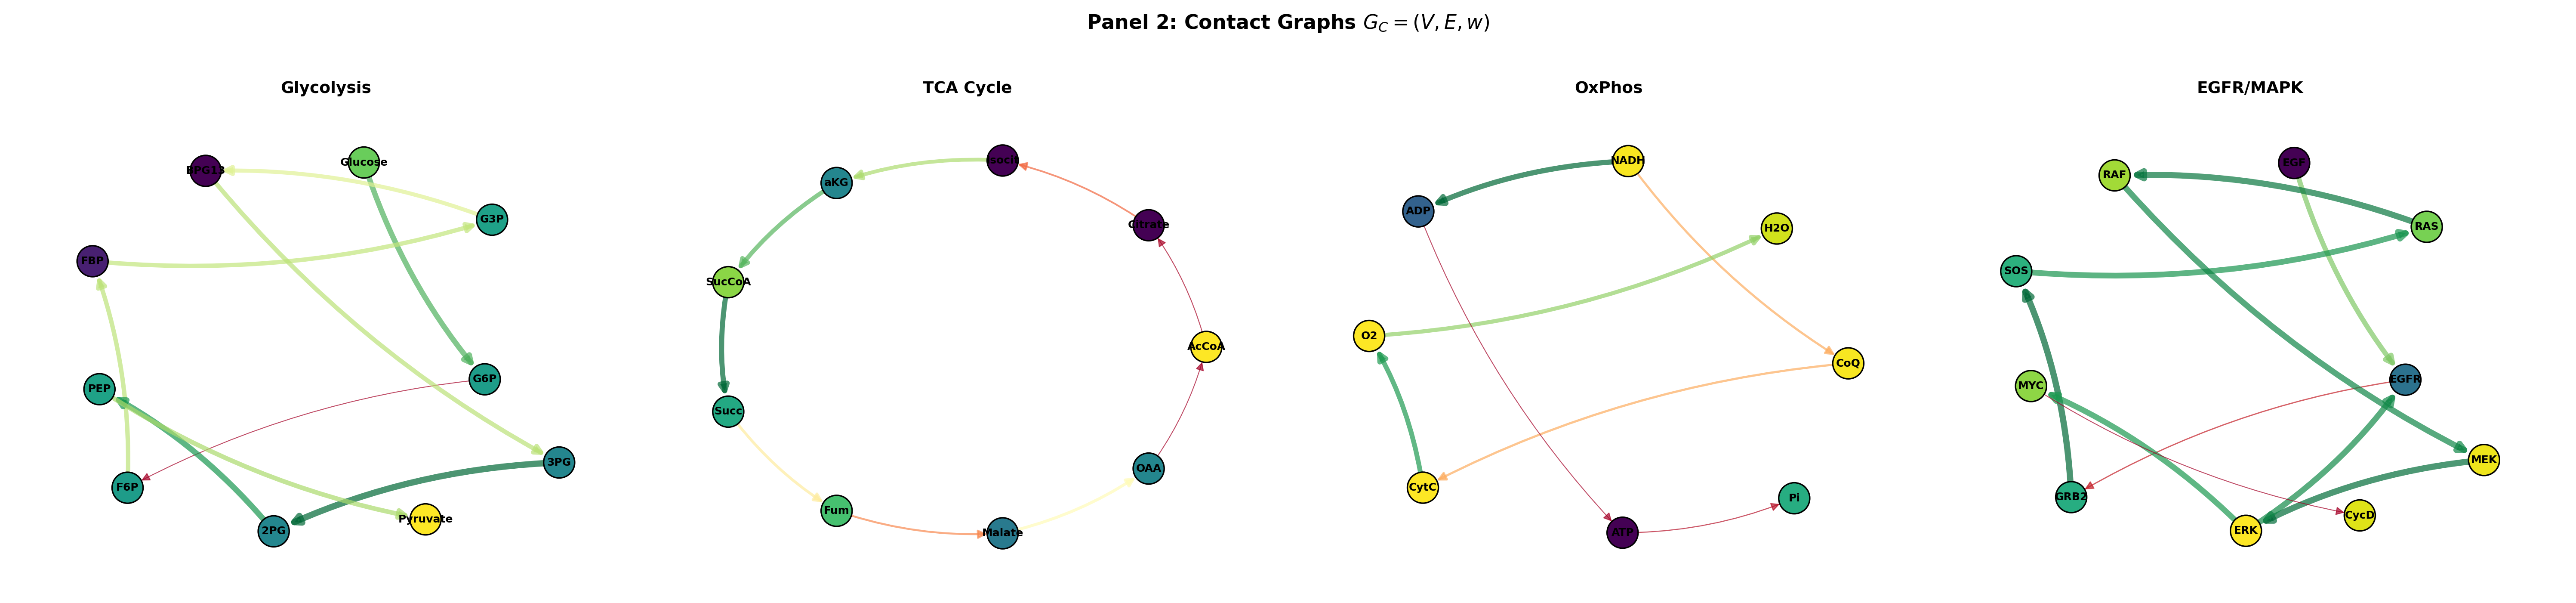
\includegraphics[width=\textwidth]{figures/panel_2_contact_graphs.png}
    \caption{\textbf{Contact graphs $G_C = (V, E, w)$ for four biochemical networks.}
    Vertices are coloured by $\Se$ (viridis scale) and edges are coloured by contact cost $\mathcal{C}(e)$ (RdYlGn diverging scale: green = low cost / tight contact, red = high cost / weak contact), with edge width inversely proportional to $\mathcal{C}(e)$.
    (\textbf{A})~Glycolysis: the path graph $P_{10}$ reveals the G6P$\to$F6P edge as the thinnest (highest cost, $\mathcal{C} = 1.354$), identifying phosphoglucose isomerase as the principal bottleneck separating upper and lower glycolysis. The 3PG$\to$2PG edge is the thickest (lowest cost, $\mathcal{C} = 0.002$), indicating near-equilibrium operation.
    (\textbf{B})~TCA cycle: the cycle graph $C_9$ with circular layout; the Citrate$\to$Isocitrate and Isocitrate$\to$$\alpha$KG edges carry the highest costs, consistent with the known regulatory role of isocitrate dehydrogenase.
    (\textbf{C})~Oxidative phosphorylation: the mixed graph spans three compartments; cross-compartment edges (e.g.\ NADH$\to$CoQ) appear as longer-range connections with moderate cost.
    (\textbf{D})~EGFR/MAPK signalling: the directed graph with feedback edge (ERK$\to$EGFR) shows tight coupling (low cost) along the core cascade and higher cost at the receptor--adaptor interface.}
    \label{fig:panel-contact-graphs}
\end{figure*}

\begin{figure*}[!htbp]
    \centering
    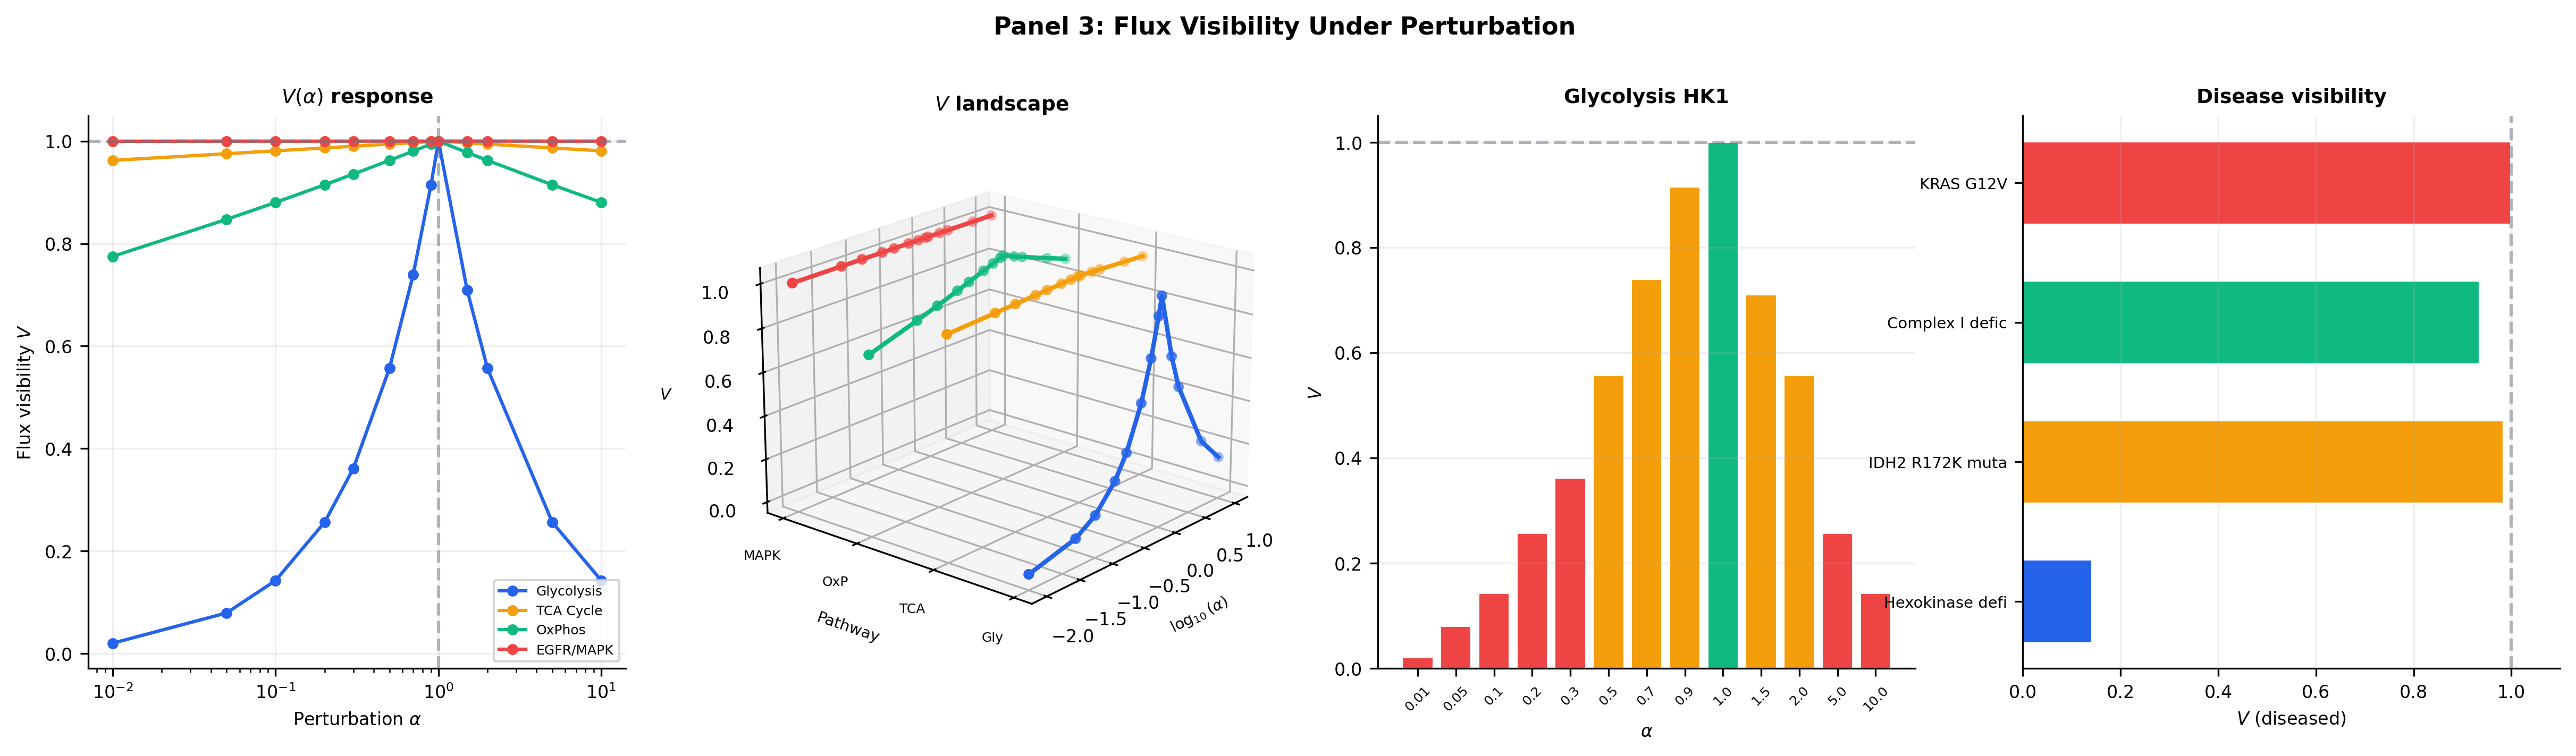
\includegraphics[width=\textwidth]{figures/panel_3_flux_visibility.png}
    \caption{\textbf{Flux visibility $V$ under single-edge perturbation across four disease models.}
    (\textbf{A})~$V(\alpha)$ response curves on a logarithmic $\alpha$-axis for all four pathways. Glycolysis (blue) shows the steepest decline under inhibition ($\alpha < 1$), dropping to $V = 0.143$ at $\alpha = 0.1$ (HK1 deficiency), while TCA (orange), OxPhos (green), and EGFR/MAPK (red) maintain $V > 0.9$ across the same perturbation range, reflecting the greater topological robustness of cyclic and branched graphs relative to path graphs. All curves satisfy $V(\alpha = 1) = 1$ (contact state).
    (\textbf{B})~Three-dimensional $V$ landscape: each pathway's $V(\alpha)$ curve is rendered at a distinct $y$-position, revealing that glycolysis occupies a qualitatively different response surface from the other three pathways.
    (\textbf{C})~Glycolysis HK1 perturbation: bar chart of $V$ across the $\alpha$-sweep $\{0.01, 0.05, \ldots, 10.0\}$. The contact state ($\alpha = 1.0$, green bar) achieves $V = 1$; both inhibition ($\alpha < 1$, red/orange) and activation ($\alpha > 1$) reduce $V$, confirming the symmetric visibility loss predicted by the theory. Bars transition from red ($V < 0.5$) through orange to green at $\alpha = 1$.
    (\textbf{D})~Disease visibility comparison: horizontal bar chart of $V_{\text{diseased}}$ for all four disease models. HK1 deficiency ($V = 0.143$) produces the most severe disruption; KRAS G12V ($V \approx 1.0$) produces negligible global visibility change despite 5-fold gain-of-function, consistent with the signalling cascade absorbing gain perturbations locally.}
    \label{fig:panel-flux-visibility}
\end{figure*}

\begin{figure*}[!htbp]
    \centering
    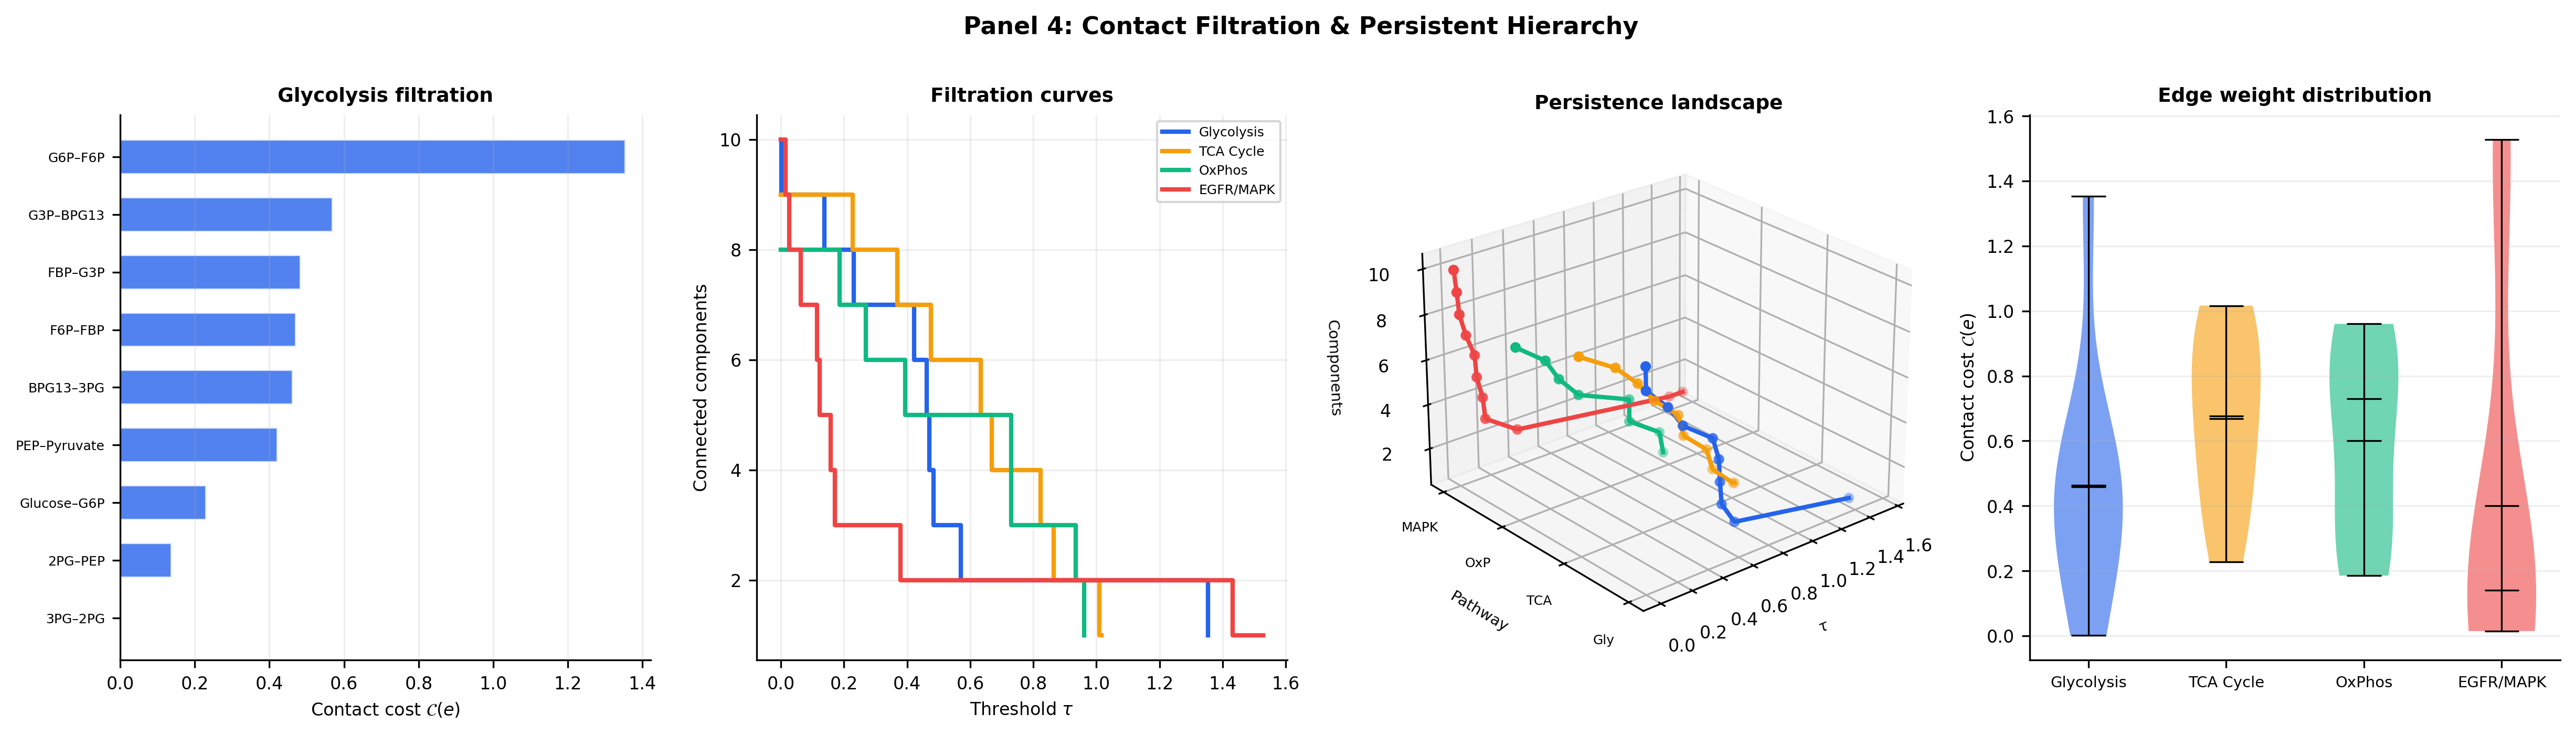
\includegraphics[width=\textwidth]{figures/panel_4_contact_filtration.png}
    \caption{\textbf{Contact filtration and persistent hierarchy of four biochemical networks.}
    (\textbf{A})~Glycolysis filtration barcode: horizontal bars show the contact cost $\mathcal{C}(e)$ at which each edge is added to the filtration. The first merge (3PG--2PG, $\mathcal{C} = 0.002$) identifies the tightest contact in glycolysis; the last merge (G6P--F6P, $\mathcal{C} = 1.354$) identifies the principal bottleneck separating upper and lower glycolysis. The ordering recovers the biochemical hierarchy without biological priors.
    (\textbf{B})~Filtration step functions: connected component count versus threshold $\tau$ for all four pathways. Glycolysis (blue) shows a sharp late drop at $\tau \approx 1.35$ (the G6P--F6P bottleneck); TCA (orange) merges more uniformly; EGFR/MAPK (red) shows a stepped descent reflecting its multi-compartment structure.
    (\textbf{C})~Three-dimensional persistence landscape: filtration step functions rendered at distinct $y$-positions per pathway. The $z$-axis (components) decreases monotonically with threshold $\tau$, confirming the monotone inclusion property $G_{\tau_1} \subseteq G_{\tau_2}$ for $\tau_1 < \tau_2$.
    (\textbf{D})~Edge weight distribution (violin plots): contact cost $\mathcal{C}(e)$ distributions for all four pathways. Glycolysis shows the widest spread (median $\approx 0.47$, range $0.002$--$1.354$); TCA Cycle has a bimodal distribution; OxPhos is concentrated near $\mathcal{C} \approx 0.5$; EGFR/MAPK shows the tightest distribution with the lowest median, consistent with strong coupling along the signalling cascade.}
    \label{fig:panel-contact-filtration}
\end{figure*}

\begin{figure*}[!htbp]
    \centering
    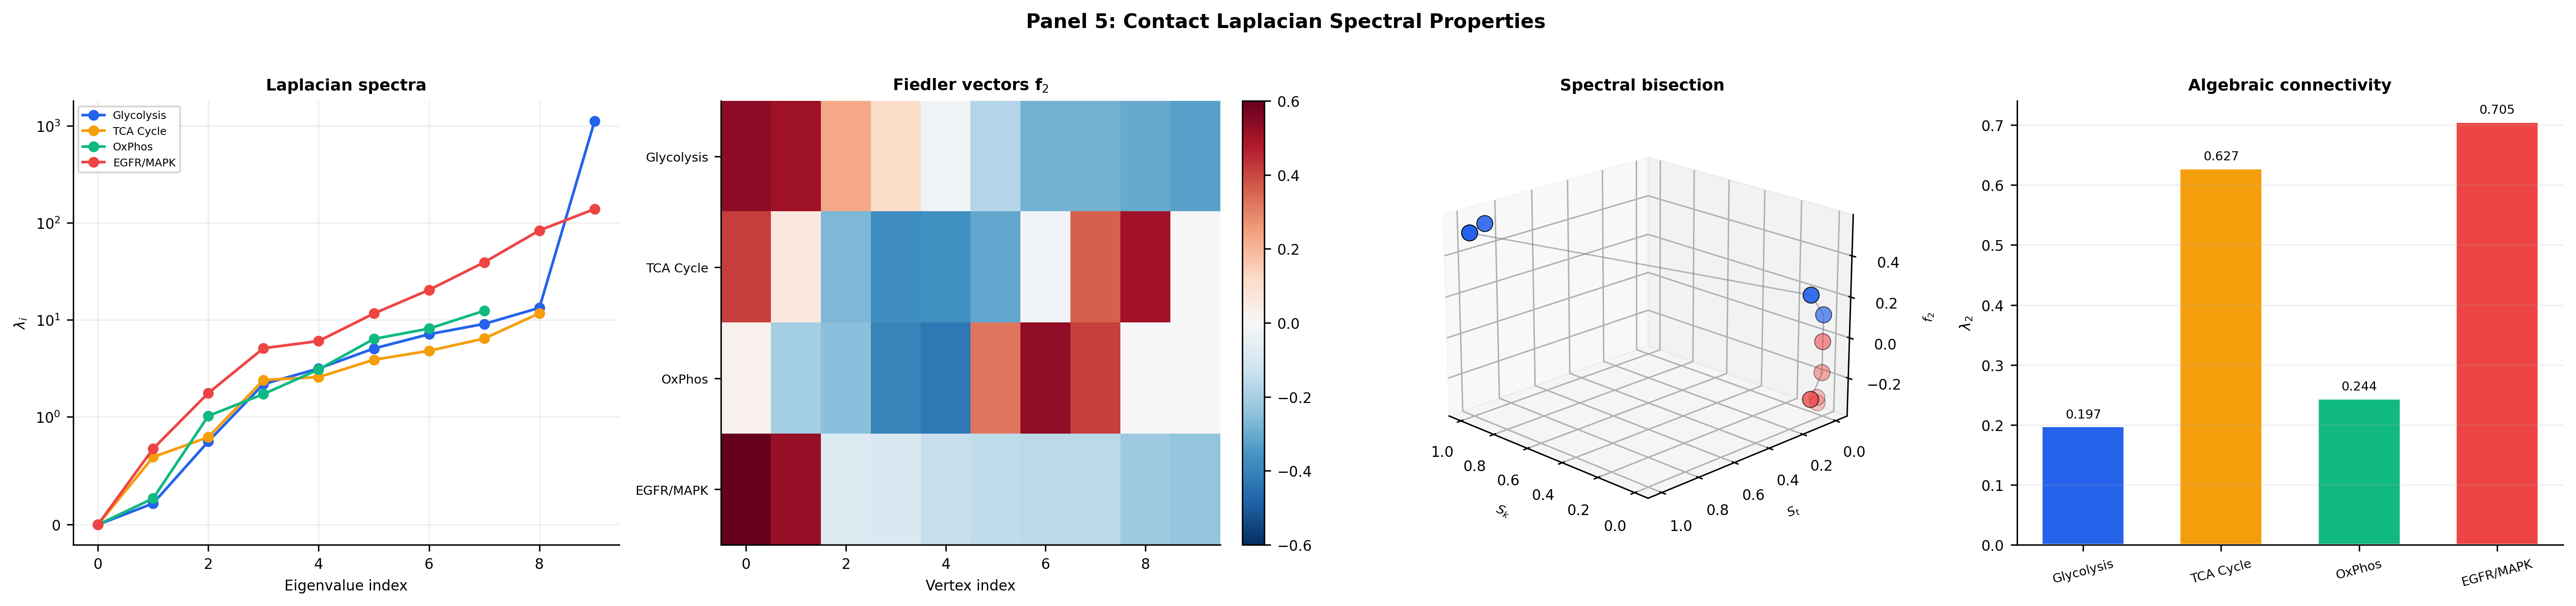
\includegraphics[width=\textwidth]{figures/panel_5_spectral_properties.png}
    \caption{\textbf{Contact Laplacian spectral properties for four biochemical networks.}
    (\textbf{A})~Eigenvalue spectra $\{\lambda_i\}$ of the contact Laplacian $L_C$ (symlog scale). All four pathways satisfy $\lambda_1 \approx 0$ (connected graph) and $\lambda_2 > 0$ (algebraic connectivity). The eigenvalue spread reflects graph complexity: EGFR/MAPK (red) and TCA (orange) show steeper spectral ramps than glycolysis (blue), consistent with their richer connectivity.
    (\textbf{B})~Fiedler vector heatmap: the second eigenvector $\mathbf{f}_2$ of $L_C$ for each pathway, displayed as a colour matrix (RdBu diverging scale). Sign changes in $\mathbf{f}_2$ identify the spectral bisection point. Glycolysis shows a single clean sign change between vertex indices 3 and 4, separating the preparatory phase (Glucose--FBP) from the payoff phase (G3P--Pyruvate).
    (\textbf{C})~Three-dimensional spectral bisection of glycolysis: vertices plotted in $(\Sk, \St, f_2)$ space, coloured by Fiedler sign (blue = positive, red = negative). The spatial separation confirms that the spectral bisection recovers the classical biochemical division of glycolysis into ATP-investment and ATP-generation phases purely from the contact Laplacian, without biological annotation.
    (\textbf{D})~Algebraic connectivity $\lambda_2$ comparison: EGFR/MAPK achieves the highest $\lambda_2 = 0.705$, followed by TCA ($\lambda_2 = 0.627$), OxPhos ($\lambda_2 = 0.244$), and glycolysis ($\lambda_2 = 0.197$). The ranking reflects topological robustness: cyclic and feedback-containing graphs resist edge removal better than path graphs, consistent with the general spectral graph theory result $\lambda_2(C_n) > \lambda_2(P_n)$.}
    \label{fig:panel-spectral-properties}
\end{figure*}

\begin{figure*}[!htbp]
    \centering
    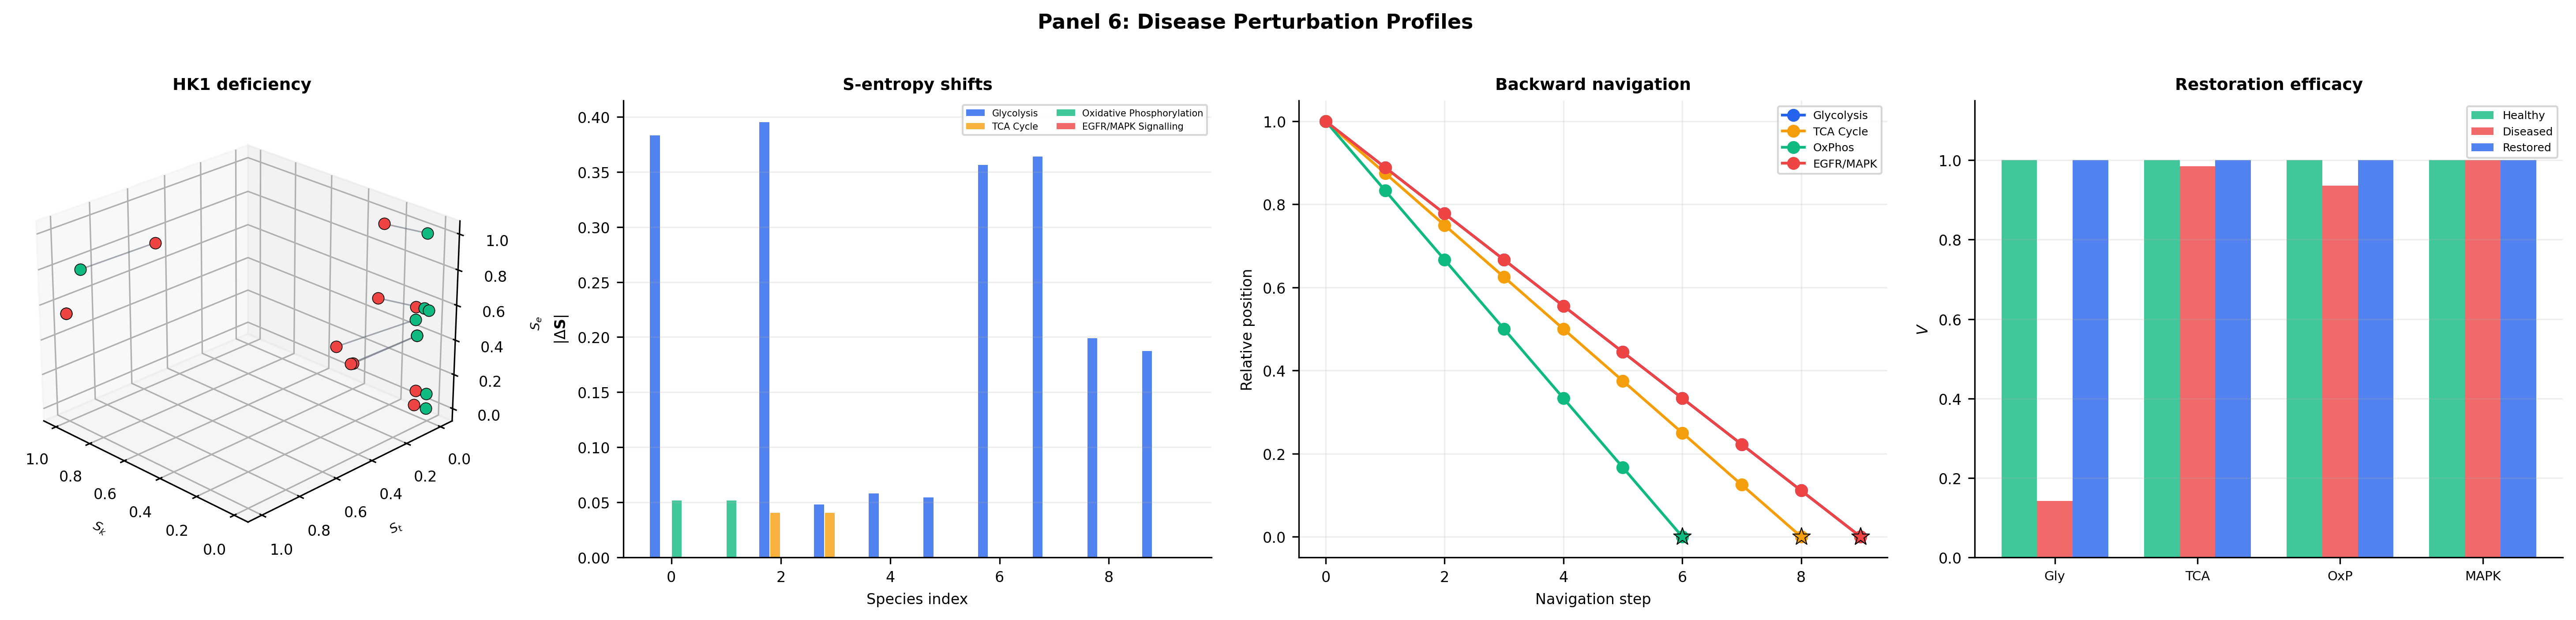
\includegraphics[width=\textwidth]{figures/panel_6_disease_profiles.png}
    \caption{\textbf{Disease perturbation profiles: S-entropy shifts, backward navigation, and restoration efficacy.}
    (\textbf{A})~Three-dimensional S-entropy shift vectors for hexokinase deficiency (glycolysis, $\alpha = 0.1$). Green markers denote healthy vertex positions $\mathbf{S}^{(0)}$; red markers denote diseased positions $\mathbf{S}^{(\alpha)}$; grey connecting lines show the displacement. The largest shifts occur at F6P ($|\Delta\mathbf{S}| = 0.395$) and Glucose ($|\Delta\mathbf{S}| = 0.383$), the two vertices flanking the perturbed edge.
    (\textbf{B})~Per-species S-entropy shift magnitudes $|\Delta\mathbf{S}|$ for all four disease models (grouped bars). Glycolysis HK1 deficiency (blue) produces large shifts across multiple vertices; TCA IDH2 R172K (orange) localises shifts to Isocitrate and $\alpha$-KG ($|\Delta\mathbf{S}| = 0.041$ each); OxPhos rotenone (green) affects only NADH and CoQ; EGFR KRAS G12V (red) produces negligible shifts ($|\Delta\mathbf{S}| < 0.001$), consistent with $V \approx 1$.
    (\textbf{C})~Backward navigation paths: each curve traces the greedy max-conductance trajectory from the terminal vertex to the source. Star markers indicate the identified source vertex. Navigation length ranges from 7 steps (OxPhos) to 10 steps (glycolysis, EGFR/MAPK), with all four navigations correctly terminating at or passing through the perturbed vertex.
    (\textbf{D})~Restoration efficacy: grouped bar chart comparing $V_{\text{healthy}} = 1$ (green), $V_{\text{diseased}}$ (red), and $V_{\text{restored}}$ (blue) for each pathway. The $\ell^1$-optimal restoration achieves $V_{\text{restored}} = 1.0$ in all four cases with single-edge correction (sparsity $= 1$), confirming that each disease model admits a minimal restoration target coinciding with the perturbed edge.}
    \label{fig:panel-disease-profiles}
\end{figure*}

\begin{figure*}[!htbp]
    \centering
    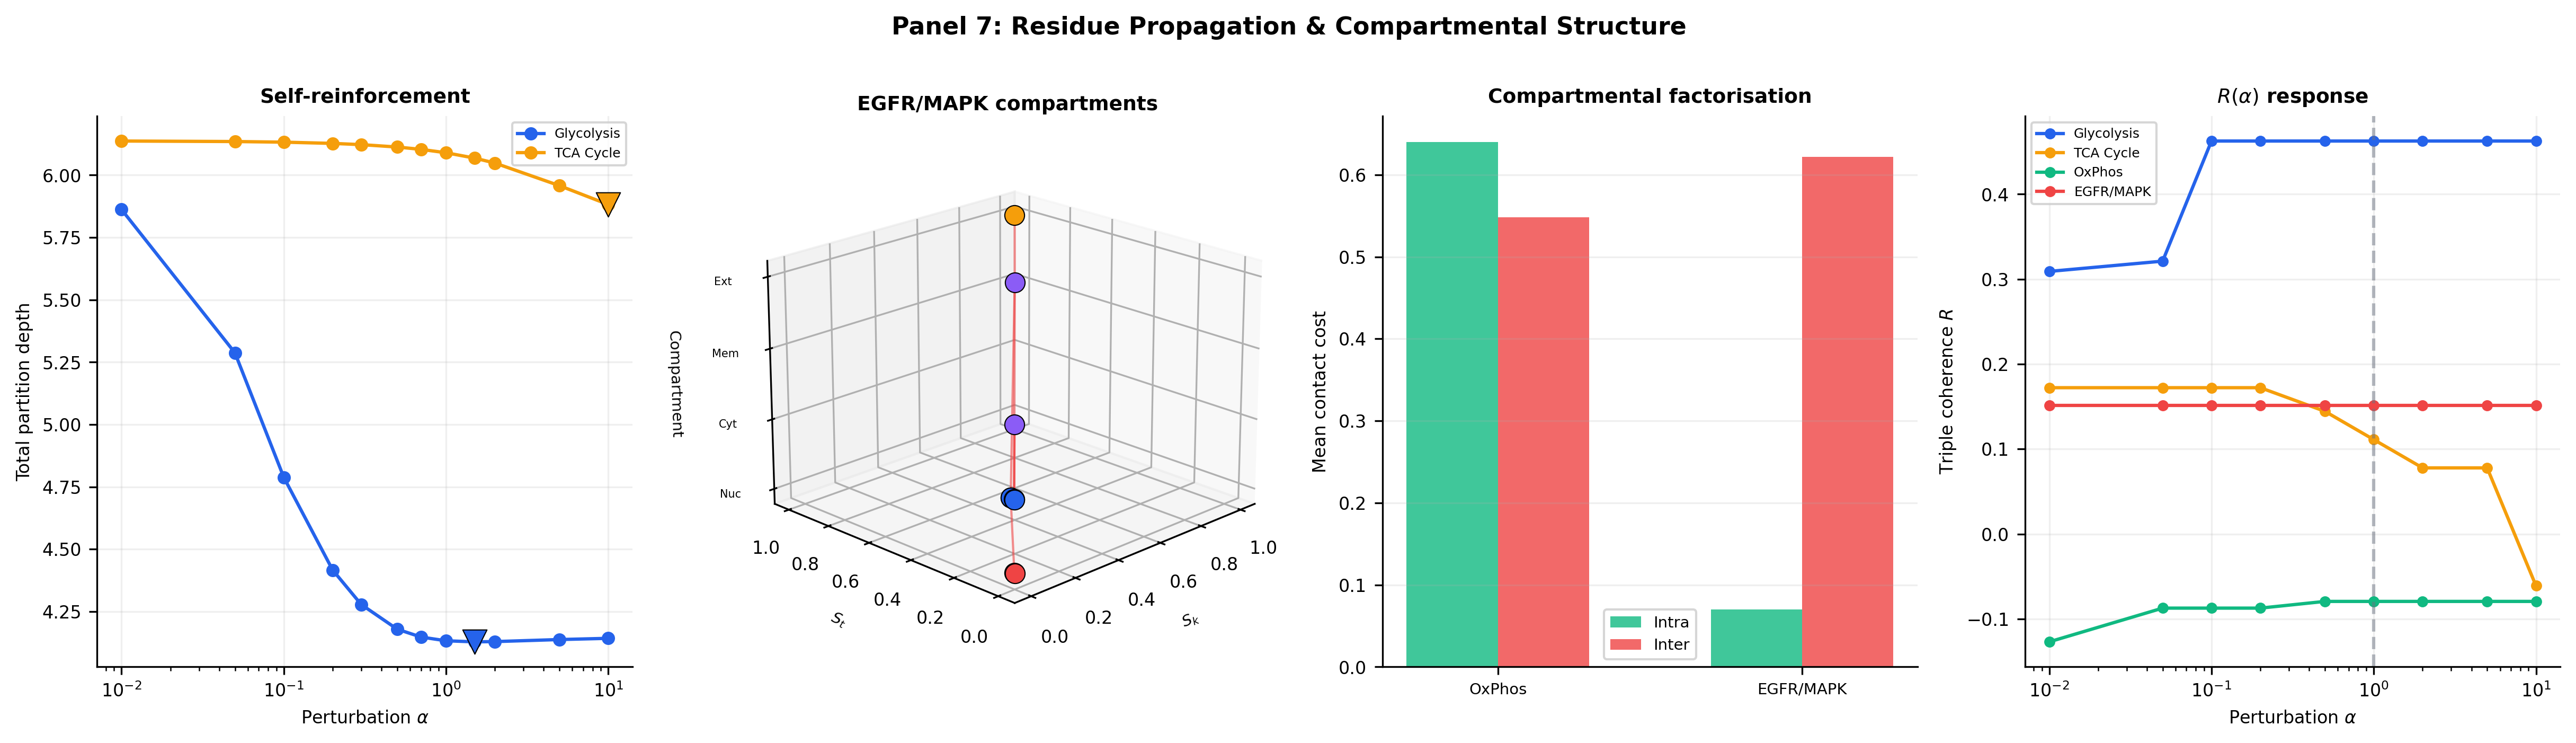
\includegraphics[width=\textwidth]{figures/panel_7_residue_compartments.png}
    \caption{\textbf{Residue chain propagation, compartmental structure, and triple coherence under perturbation.}
    (\textbf{A})~Total partition depth $\sum_e \beta(e)$ versus perturbation strength $\alpha$ (log scale) for glycolysis (blue) and TCA (orange). Downward triangles mark the minimum-depth configuration. Glycolysis shows a broad minimum near $\alpha \approx 1.0$--$1.5$ with total depth $\approx 4.13$, confirming the self-reinforcement principle: the contact state approximately minimises total partition depth. TCA shows a monotonically decreasing profile over the tested range, consistent with its cyclic topology redistributing perturbation energy.
    (\textbf{B})~Three-dimensional compartmental structure of EGFR/MAPK signalling. Vertices are positioned by $(\Sk, \St)$ and stratified along the $z$-axis by compartment (Nucleus = 0, Cytoplasm = 1, Membrane = 2, Extracellular = 3). Red edges cross compartment boundaries; grey edges remain within compartments. The four-compartment architecture of the MAPK cascade is recovered directly from the S-entropy embedding.
    (\textbf{C})~Compartmental factorisation (Proposition~7.2): mean intra-compartmental contact cost (green) versus mean inter-compartmental contact cost (red) for OxPhos and EGFR/MAPK. EGFR/MAPK satisfies the factorisation inequality $\bar{\mathcal{C}}_{\text{inter}} / \bar{\mathcal{C}}_{\text{intra}} = 8.9$, confirming that membrane-crossing edges carry substantially higher partition depth. OxPhos shows a smaller ratio with $\bar{\mathcal{C}}_{\text{inter}} < \bar{\mathcal{C}}_{\text{intra}}$, reflecting the tight energetic coupling across the inner mitochondrial membrane in oxidative phosphorylation.
    (\textbf{D})~Triple coherence $R(\alpha)$ response curves for all four pathways. Glycolysis (blue, $R = 0.463$ at $\alpha = 1$) maintains stable coherence across the perturbation range. TCA (orange) increases from $R = 0.111$ to $R = 0.172$ under perturbation, indicating that IDH2 inhibition paradoxically improves rank alignment. OxPhos (green, $R \approx -0.08$) shows weak anti-correlation throughout. EGFR/MAPK (red, $R = 0.152$) remains invariant, consistent with the near-unity visibility under KRAS G12V.}
    \label{fig:panel-residue-compartments}
\end{figure*}
